\documentclass{article}
\usepackage[margin=1cm,landscape]{geometry}
\usepackage{tikz}
\usetikzlibrary{positioning,arrows.meta}
\pagestyle{empty}
\begin{document}
\begin{center}
\Large CarbonDesk: Guillermo's emissions classes\par\medskip
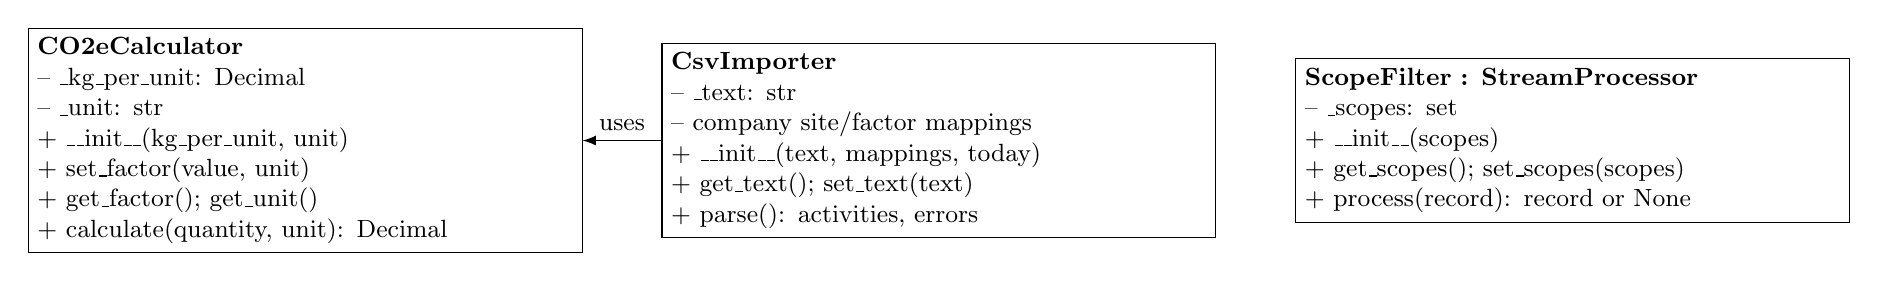
\begin{tikzpicture}[box/.style={draw,rectangle,align=left,text width=6.8cm,font=\small},>=Latex]
\node[box] (calc) {\textbf{CO2eCalculator}\\
-- \_kg\_per\_unit: Decimal\\-- \_unit: str\\
+ \_\_init\_\_(kg\_per\_unit, unit)\\+ set\_factor(value, unit)\\+ get\_factor(); get\_unit()\\+ calculate(quantity, unit): Decimal};
\node[box,right=1cm of calc] (csv) {\textbf{CsvImporter}\\
-- \_text: str\\-- company site/factor mappings\\
+ \_\_init\_\_(text, mappings, today)\\+ get\_text(); set\_text(text)\\+ parse(): activities, errors};
\node[box,right=1cm of csv] (filter) {\textbf{ScopeFilter : StreamProcessor}\\
-- \_scopes: set\\+ \_\_init\_\_(scopes)\\+ get\_scopes(); set\_scopes(scopes)\\+ process(record): record or None};
\draw[->] (csv) -- node[above,font=\small]{uses} (calc);
\end{tikzpicture}
\par\bigskip
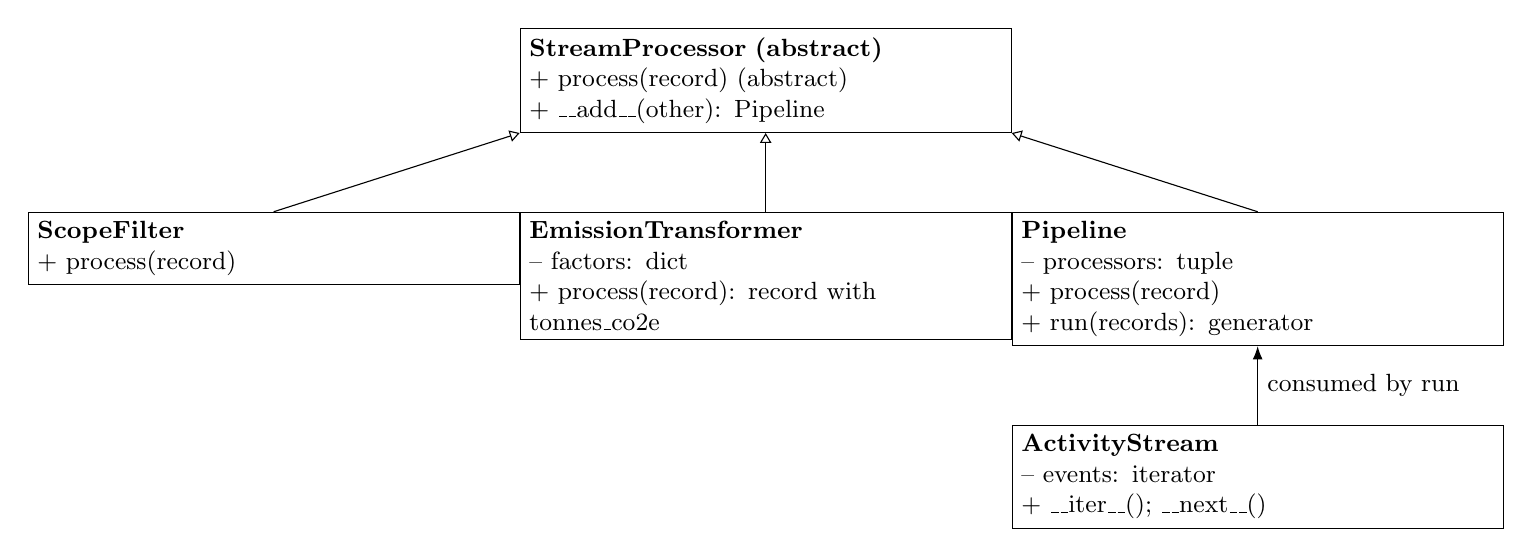
\begin{tikzpicture}[box/.style={draw,rectangle,align=left,text width=6cm,font=\small},>=Latex]
\node[box] (abc) {\textbf{StreamProcessor (abstract)}\\+ process(record) (abstract)\\+ \_\_add\_\_(other): Pipeline};
\node[box,below left=1cm and 0cm of abc] (f) {\textbf{ScopeFilter}\\+ process(record)};
\node[box,below=1cm of abc] (t) {\textbf{EmissionTransformer}\\-- factors: dict\\+ process(record): record with tonnes\_co2e};
\node[box,below right=1cm and 0cm of abc] (p) {\textbf{Pipeline}\\-- processors: tuple\\+ process(record)\\+ run(records): generator};
\draw[-{Triangle[open]}] (f.north) -- (abc.south west);
\draw[-{Triangle[open]}] (t.north) -- (abc.south);
\draw[-{Triangle[open]}] (p.north) -- (abc.south east);
\node[box,below=1cm of p] (s) {\textbf{ActivityStream}\\-- events: iterator\\+ \_\_iter\_\_(); \_\_next\_\_()};
\draw[->] (s) -- node[right,font=\small]{consumed by run} (p);
\end{tikzpicture}
\end{center}
\end{document}
